\section{关于期权的其他结果}
\begin{enumerate}[label=\arabic{section}.\arabic*]
    \item \sol\\ 成立.
    \item \sol\\ 服从一个漂移参数为$\displaystyle r-\frac{\sigma^2}{2}-f$,波动参数为$\sigma$的几何布朗运动.
    \item \sol\\ $C(s(1-f)^2,K,t,r,\sigma)$.
    \item \pro\\ 在没有分红时,不应该提前执行看涨期权,所以不应该在$t_d$之前或在$(t_d, t)$之间执行看涨期权,即所证.
    \item \sol\\ 上限期权的收益是$(K,t)$看涨期权和$(K+B,t)$看涨期权收益的差,因此,根据一价律,无套利价格为$C(s,K, t, r, \sigma) - C(s,K + B, t, r, \sigma)$.
    \item \sol\\ 在风险中性几何布朗运动下,该投资的预期收益为
    \[E[(1+\beta)s+\alpha(S(1)-(1+\beta)s)^+]=(1+\beta)s+\alpha\e^{r}C(s,t,(1+\beta)s,\sigma,r),\]
    由于无套利存在,所以上式等于$s\e^r$,可解得
    \[\alpha=\frac{s(\e^r-1-\beta)}{\e^rC(s,t,(1+\beta)s,\sigma,r)}.\]
    \item \pro\\ 在风险中性几何布朗运动下,当$K>(1+\beta)s$时,该投资的预期收益为
    \[E[(1+\beta)s+(S(1)-(1+\beta)s)^+-(S(1)-K)^+] = (1+\beta)s+\e^rC(s, t, (1+\beta)s, \sigma, r)-\e^rC(s, t,K, \sigma, r),\]
    由于无套利存在,所以上式等于$s\e^r$,化简即可得
    \[C(s, 1,K, \sigma, r)=C(s, 1, s(1+\beta), \sigma, r)+s(1+\beta)\e^{-r}-s.\]
    同时,因为$s(1+\beta)\e^{-r}-s<0$,而$C(s, t,K, \sigma, r)$关于$K$递减,所以$K>(1+\beta)s$一定成立,即上式必成立.
    \item \pro \begin{align*}
        C(s\e^{-ft},t,K,\sigma,r)&=\e^{-rt}E[(s\e^{-ft}\e^W-K)^+]=\e^{-rt}E[(s\e^{-ft}\e^{\sigma\sqrt{t}Z+(r-\sigma^2/2)t}-K)^+]\\
        &=\e^{-rt}E[(s\e^{\sigma\sqrt{t}Z+(r-f-\sigma^2/2)t}-K)^+]\\
        &=\e^{-rt}\e^{-(r-f)t}E[(s\e^{\sigma\sqrt{t}Z+(r-f-\sigma^2/2)t}-K)^+]\\
        &=\e^{-rt}C(s,t,K,\sigma,r-f)
    \end{align*}
    \item \pro
    \begin{enumerate}[label=\alph*)]
        \item 比起在时刻$s<t_1$执行看涨期权支付$K_1$,显然在时刻$t_1$执行看涨期权支付$K_1$会更好.
        \item 因为在时刻$t_1$,看涨期权的价格为$C(x,t-t_1,K,\sigma,r)$,同时$S(t_1)=x$.
        \item 因为$C(y,t-t_1,K,\sigma,r)$关于$y$严格单调递增.
        \item 因为在时刻$t_1$行使购买看涨期权的期权是最佳策略当且仅当$S(t_1) \geq x$.
    \end{enumerate}
    \item \pro
    \begin{enumerate}[label=\alph*)]
        \item 若在时刻$t_2$执行期权,支付$K_2\e^{-rt_2}$;若在时刻$t_1$执行期权,支付$K_1\e^{-rt_1}$. 因为$K_1>\e^{-r(t_2-t_1)}K_2 \Rightarrow K_2\e^{-rt_2}<K_1\e^{-rt_1}$,所以不应该在时刻$t_1$执行期权.
        \item 若在时刻$t_1$期权不执行且$S(t_1)=y$,此时的风险中性收益为$C(y,t_2-t_1,K_2,\sigma,r)$. 若在时刻$t_1$期权执行,此时的收益为$y-K_1$. 所以当$S(t_1)=y$时,若$C(y,t_2-t_1,K_2,\sigma,r)<y-K_1$则应该在时刻$t_1$执行期权,证毕.
    \end{enumerate}
    \item \sol
    \begin{figure}[H]
        \centering
        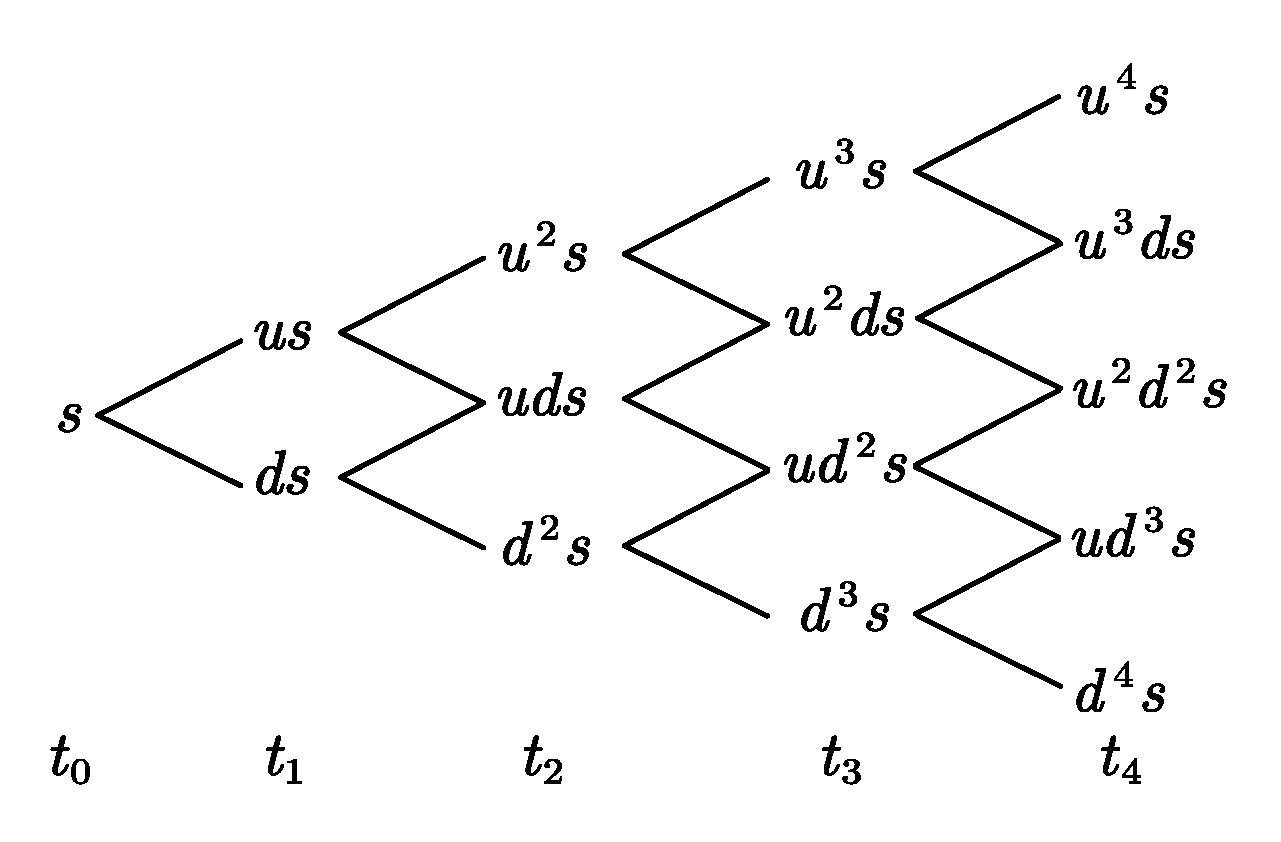
\includegraphics[scale=0.35]{8.11.pdf}
    \end{figure}
    \item \sol
    \begin{enumerate}[label=\alph*)]
        \item 正确,原因略.
        \item 错误,原因略.
        \item 错误,原因略.
        \item 正确,原因略.
    \end{enumerate}
    \item \sol\\
    本题中的参数为\[t=\frac{1}{4},r=0.06,\sigma=0.3,K=10,S(0)=s=9,\]
    则\[\omega=\frac{rt+\sigma^2t/2-\ln[K/S(0)]}{\sigma\sqrt{t}}=\frac{0.06/4+0.3^2/8-\ln(10/9)}{0.3/\sqrt{4}}=-0.5274,\]
    而$\Phi(-0.5274)=0.2990,\Phi(-0.6774)=0.2491$,所以
    \[P=S(0)\Phi(\omega)-K\e^{-rt}\Phi(\omega-\sigma\sqrt{t})+K\e^{-rt}-s=9\times0.2990-10\e^{-0.06/4}\times0.2491+10\e^{-0.06/4}-9=1.0882.\]
    \item \sol\\
    取$n=5$,利用参数,有
    \[u=e^{0.3\sqrt{0.05}}=1.0964,d=e^{-0.3\sqrt{0.05}}=0.9351,p=0.5056,1-p=0.4944,\beta=e^{-rt/n}=0.997,\]
    在时刻$t_5$该证券所有可能的价格是\[10d^5=7.150,10ud^4=8.383,10u^2d^3=9.829,10u^id^{5-i}>10(i=3,4,5),\]
    因此\[V_5(0)=2.850,V_5(1)=1.162,V_5(2)=0.171,V_5(i)=0(i=3,4,5),\]
    所以\begin{align*}
        V_4(2)&=\max\{1,\beta p V_5(2)+\beta(1-p)V_5(1)\}=1,V_4(1)=10-10ud^3=1.035,\\
        V_4(0)&=10-10d^4=2.354,V_4(3)=\beta p V_5(4)+\beta(1-p)V_5(3)=0,V_4(4)=0
    \end{align*}
    类似地
    \begin{align*}
        V_3(0)&=1.682,V_3(1)=1.014,V_3(2)=0.493,V_3(3)=0,\\
        V_2(0)&=1.340,V_2(1)=1.014,V_2(2)=0.243,\\
        V_1(0)&=1.172,V_1(1)=0.622,\\
        V_0(0)&=0.891
    \end{align*}
    即,看跌期权的风险中性价格近似为0.891.
    \item \sol\\ 当价格大于$K$时,应执行期权. 可通过第3章中导出的布朗运动最大时间$t$公式来定价. 它可以用$N$周期二项模型来近似,采用与美式看跌期权定价相同的状态,从后往前递推出$V_0(0)$. 与确定美式看跌期权的风险中性价格相比,因为美式资产的最优策略或无价值看涨期权是已知的,它的工作量会少一点.
    \item \omitted
    \item \sol
    \begin{enumerate}
        \item Matlab代码如下:
        \begin{lstlisting}
% 导入数据
C = ...; X = [];
for i = 1:length(C) - 1
    X(i) = log(C(i + 1) / C(i));
end
sqrt(sum(X - mean(X)) / (length(X) - 1)) * sqrt(252)
        \end{lstlisting}
        所以此时的$\sigma$的估计值为$1.2767 \times 10^{-8}$.
        \item Matlab代码如下:
        \begin{lstlisting}
% 导入数据
O = ...; C = ...;
num = 0;
for i = 1:length(C) - 1
    num = num + (log(C(i + 1)) - log(O(i + 1))) ^ 2 + (log(C(i)) - log(O(i + 1))) ^ 2;
end
sqrt(252 * num / (length(C) - 1))
        \end{lstlisting}
        所以此时的$\sigma$的估计值为0.7181.
        \item Matlab代码如下:
        \begin{lstlisting}
% 导入数据
O = ...; H = ...; L = ...; C = ...;
num = 0;
for i = 1:length(C) - 1
    num = num + 0.5 * (log(max(H)) - log(max(L))) ^ 2 - 0.39 * (log(C(i + 1)) - log(O(i + 1))) ^ 2 + (log(C(i)) - log(O(i + 1))) ^ 2;
end
sqrt(252 * num / (length(C) - 1))
        \end{lstlisting}
        所以此时的$\sigma$的估计值为0.6003.
    \end{enumerate}
\end{enumerate}
\clearpage